\documentclass{article}
\usepackage{graphicx}
\usepackage{grffile}

\usepackage{geometry}
\usepackage[MeX]{polski}
\usepackage[polish]{babel}
\usepackage{float}
\usepackage{fancyhdr}
\newcommand{\q}[1]{„#1“}
\usepackage{caption}
\usepackage{xcolor}
\usepackage[most]{tcolorbox}
\usepackage[scaled=0.85]{FiraMono} 

\usepackage[T1]{fontenc}
\usepackage{listings}
\usepackage[utf8]{inputenc}
\setlength{\parindent}{0pt} 

\newtcblisting{mylisting}{
    center,
    arc=2mm,
    top=0mm,
    bottom=0mm,
    left=3mm,
    right=0mm,
    width=\textwidth,
    boxrule=1pt,
    colback=black!85,
    listing only,
    listing options={
        basicstyle=\small\ttfamily\color{white},  
        showstringspaces=false,
        language=Java,
        keywordstyle=\color{myorange},
        stringstyle=\color{mygreen},
        commentstyle=\color{mygray}
    },
    fonttitle=\bfseries
}

\newtcblisting{mylistingXML}{
    center,
    arc=2mm,
    top=0mm,
    bottom=0mm,
    left=3mm,
    right=0mm,
    width=\textwidth,
    boxrule=1pt,
    colback=black!85,
    listing only,
    listing options={
        basicstyle=\small\ttfamily\color{white},  
        showstringspaces=false,
        language=XML,
        keywordstyle=\color{myorange},
        stringstyle=\color{mygreen},
        commentstyle=\color{mygray}
    },
    fonttitle=\bfseries
}

\renewcommand{\labelenumii}{\arabic{enumi}.\arabic{enumii}}
\renewcommand{\labelenumiii}{\arabic{enumi}.\arabic{enumii}.\arabic{enumiii}}
\renewcommand{\labelenumiv}{\arabic{enumi}.\arabic{enumii}.\arabic{enumiii}.\arabic{enumiv}}

\definecolor{mygreen}{RGB}{26, 171, 26}
\definecolor{myorange}{RGB}{230,110,20}
\definecolor{mygray}{RGB}{100,100,100}


\tcbuselibrary{listings}

\begin{document}
\begin{center}\vspace{-1cm}
    \textbf{ \Huge }\\
    \LARGE Aplikacje mobilne\\
    \large \today \\~\\
\end{center}

\begin{enumerate}
\item Aplikacja typu lista-szczegóły
\begin{enumerate}
\item Aplikacja składa się z dwóch aktywności: głównej wyświetlającej listę potraw oraz aktywności szczegółów uruchamianej po kliknięciu wybranej potrawy z listy i wyświetlającej co najmniej listę składników oraz sposób przygotowania potrawy.
Kod jest napisany w Kotlinie z wykorzystaniem fragmentów.

\begin{enumerate}

\item Aktywność wyświetlająca listę potraw.
\begin{mylisting}
class RecipeListFragment : Fragment() {
    private var _binding: FragmentRecipeListBinding? = null
    private val binding get() = _binding!!

    override fun onCreateView(
        inflater: LayoutInflater, container: ViewGroup?,
        savedInstanceState: Bundle?,
    ): View {
        _binding = FragmentRecipeListBinding.inflate(inflater, container, false)
        return binding.root
    }

    override fun onViewCreated(view: View, savedInstanceState: Bundle?) {
        super.onViewCreated(view, savedInstanceState)

        val recyclerView: RecyclerView = binding.itemList

        val itemDetailFragmentContainer: View? = 
        view.findViewById(R.id.item_detail_nav_container)

        setupRecyclerView(recyclerView, itemDetailFragmentContainer)
    }
}
\end{mylisting}

\newpage
\item Wyświetlanie listy przepisów i pobieranie ich z serwera.
\begin{mylisting}
private fun setupRecyclerView(
    recyclerView: RecyclerView,
    itemDetailFragmentContainer: View?,
) {
    RetrofitInstance.api.getRecipes().enqueue(object : retrofit2.Callback<List<Recipe>> {
        override fun onResponse(
            call: retrofit2.Call<List<Recipe>>,
            response: retrofit2.Response<List<Recipe>>,
        ) {
            if (response.isSuccessful && response.body() != null) {
                val recipes = (response.body())!!
                for (recipe in recipes) {
                    Log.e(ContentValues.TAG, recipe.title)
                }
                recyclerView.adapter = SimpleItemRecyclerViewAdapter(
                    recipes, itemDetailFragmentContainer
                )
            } else {
                Log.e(ContentValues.TAG, "Response not successful")
            }
        }

        override fun onFailure(call: retrofit2.Call<List<Recipe>>, t: Throwable) {
            Log.e(ContentValues.TAG, "Response not successful")
        }
    })
}
\end{mylisting}

\end{enumerate}

\newpage
\item Osobna wersja dla smartfonów i tabletów.

\begin{figure}[ht]
    \centering
    \begin{minipage}[b]{0.4\textwidth}
        \centering
        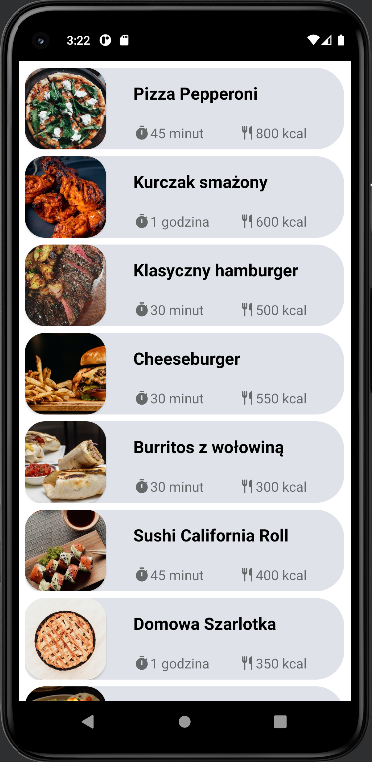
\includegraphics[width=\textwidth]{../res/phone_list}
    \end{minipage}%
    \begin{minipage}[b]{0.4\textwidth}
        \centering
        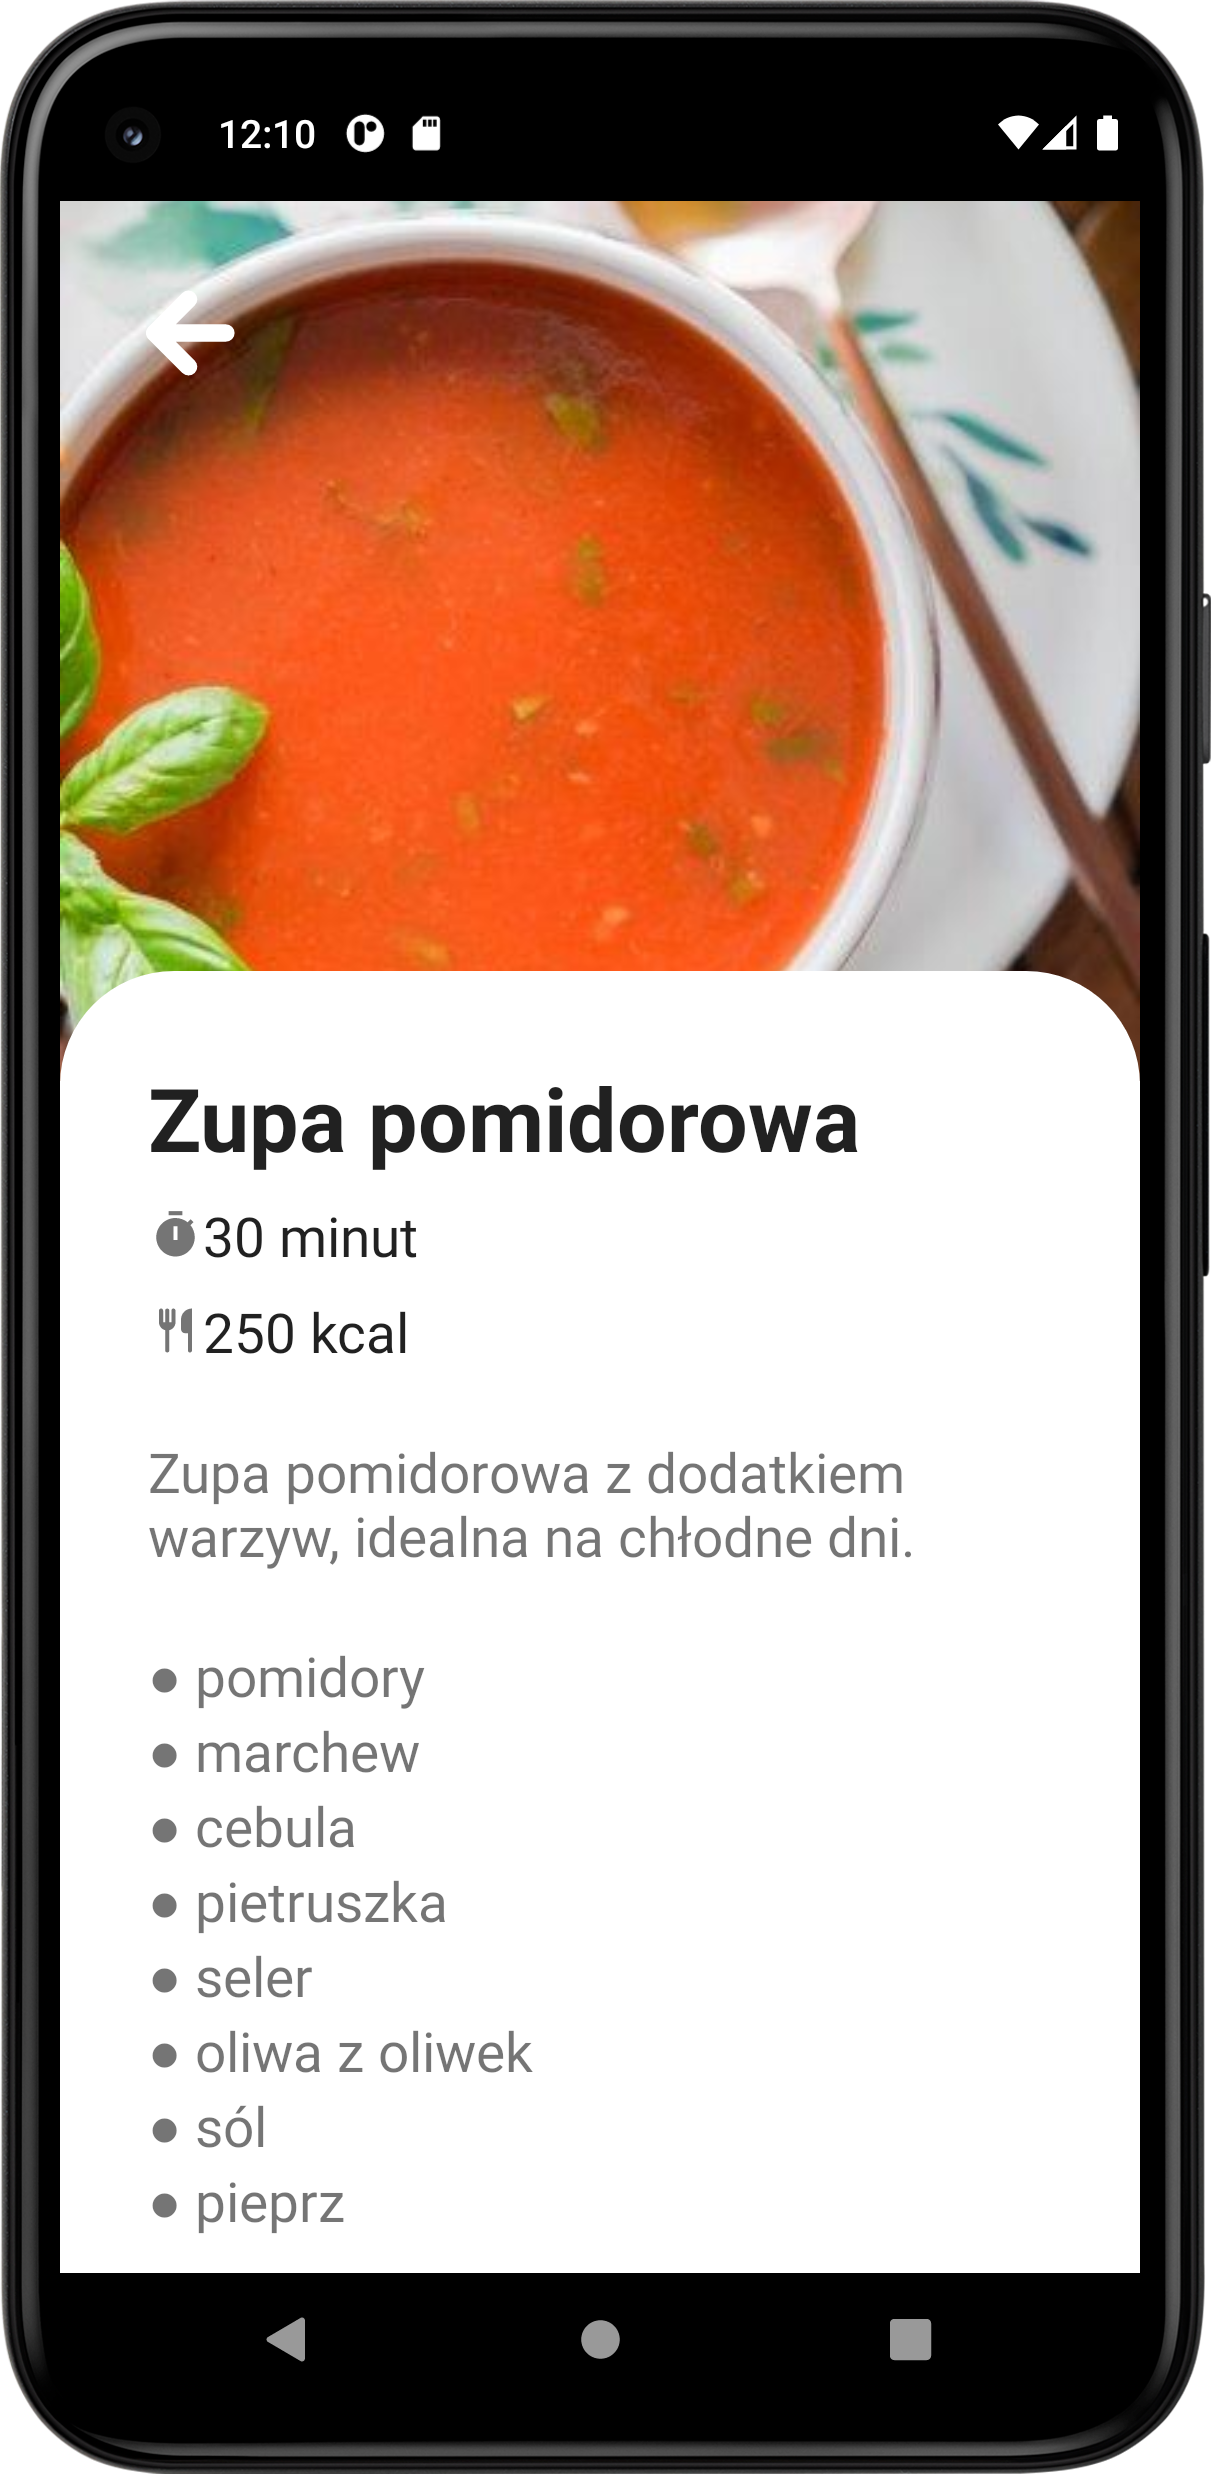
\includegraphics[width=\textwidth]{../res/phone_recipe_detail}
    \end{minipage}
    \captionof{figure}{Wersja dla smartfonów}
\end{figure}



\newpage
\begin{figure}[ht]
    \centering
    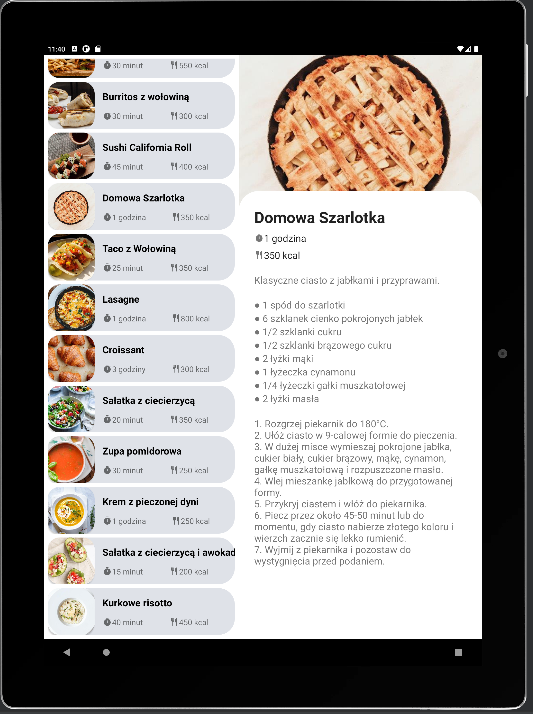
\includegraphics[width=0.7\textwidth]{../res/tablet_recipe_vertical}
    \captionof{figure}{Wersja dla tabletów}
\end{figure}
\newpage

\item Aplikacja działa po zmianie orientacji urządzenia

\begin{figure}[ht]
    \centering
    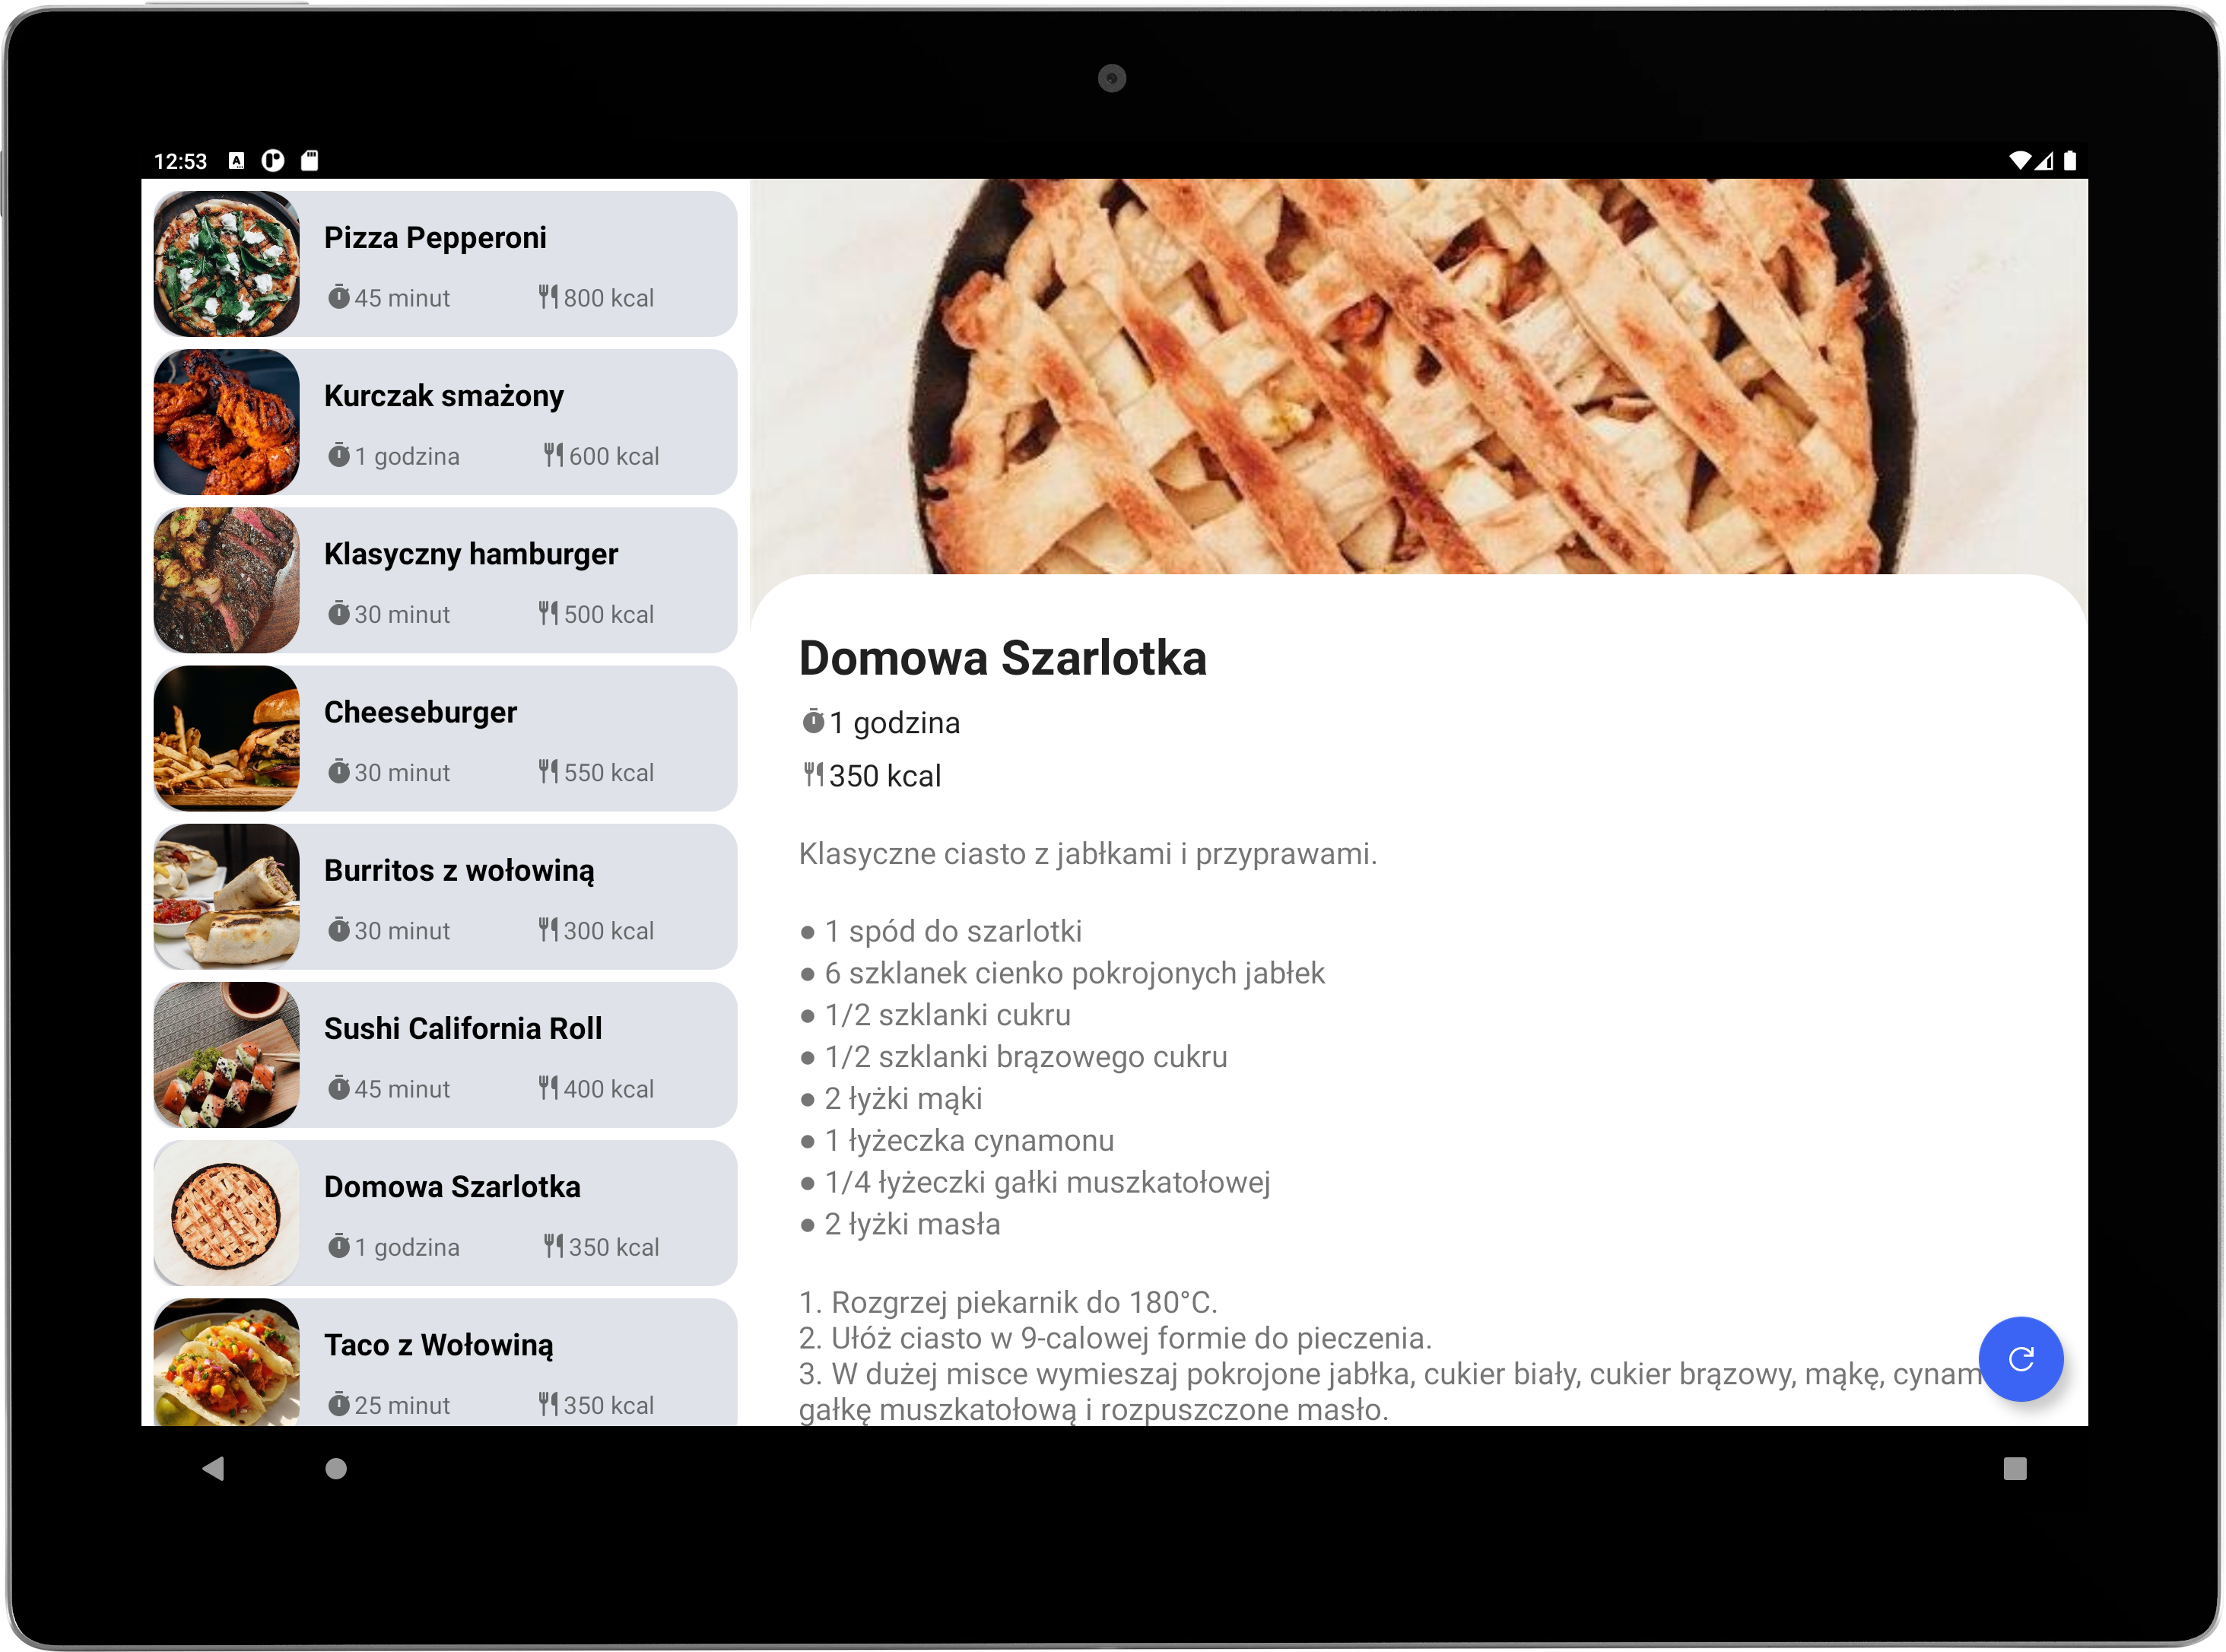
\includegraphics[width=0.7\textwidth]{../res/tablet_recipe_horizontal}
    \captionof{figure}{Wersja dla tabletów w orientacji poziomej}
\end{figure}

\begin{figure}[ht]
    \centering
    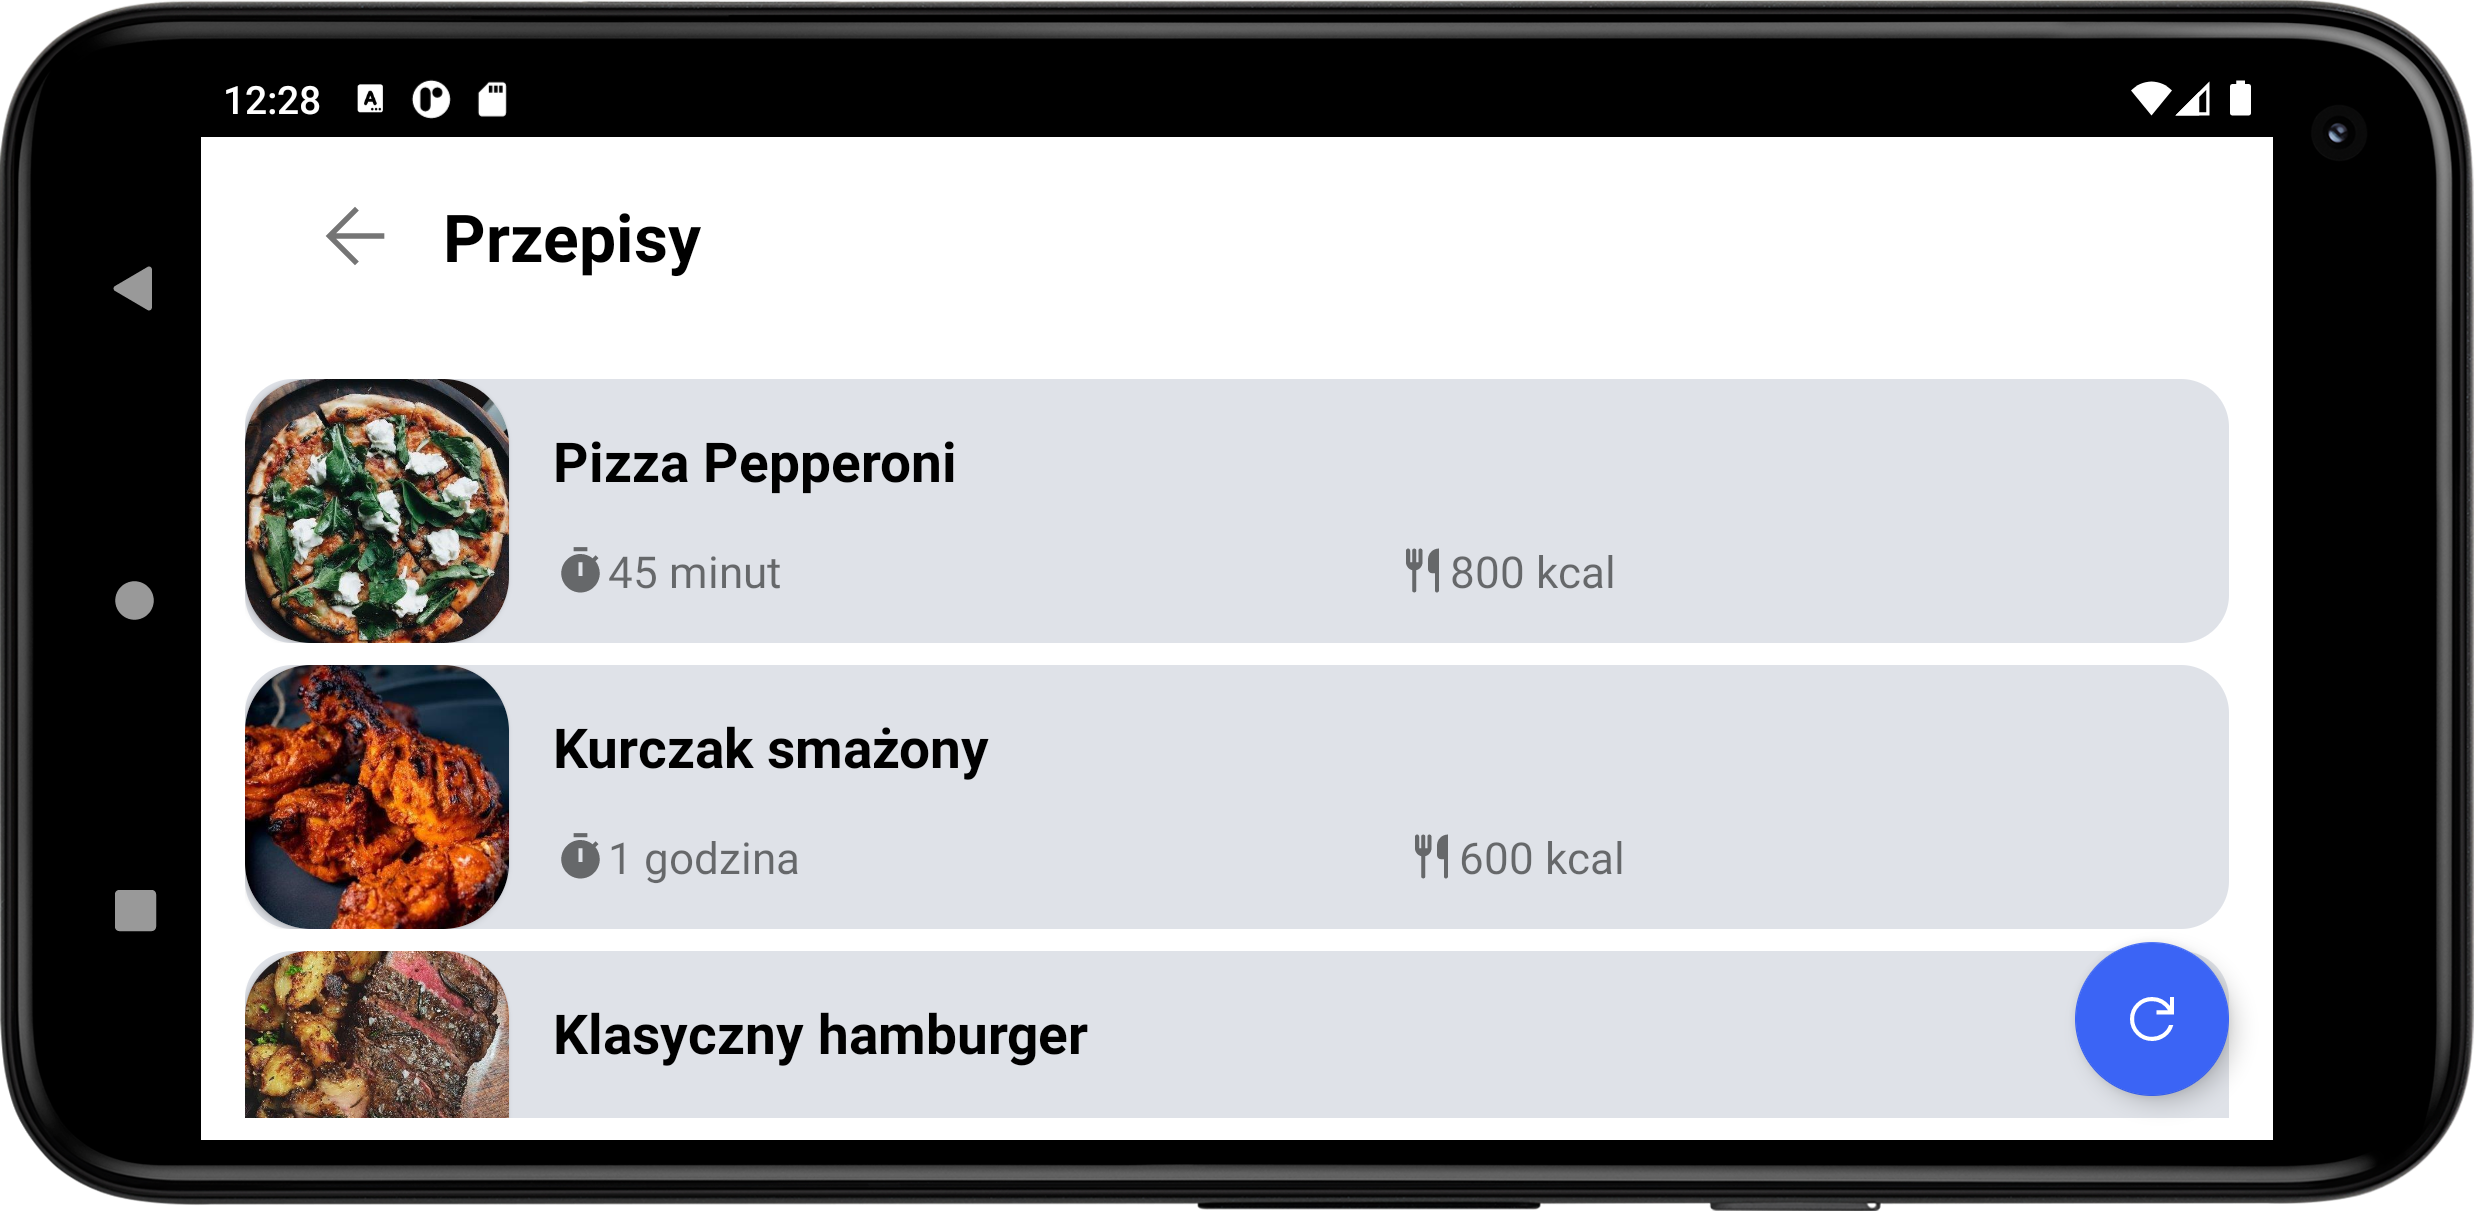
\includegraphics[width=0.45\textwidth]{../res/phone_list_horizontal}
    \captionof{figure}{Wersja dla telefonów w orientacji poziomej}
\end{figure}
\end{enumerate}

\newpage
\item Dodanie timera
\begin{figure}[ht]
    \centering
    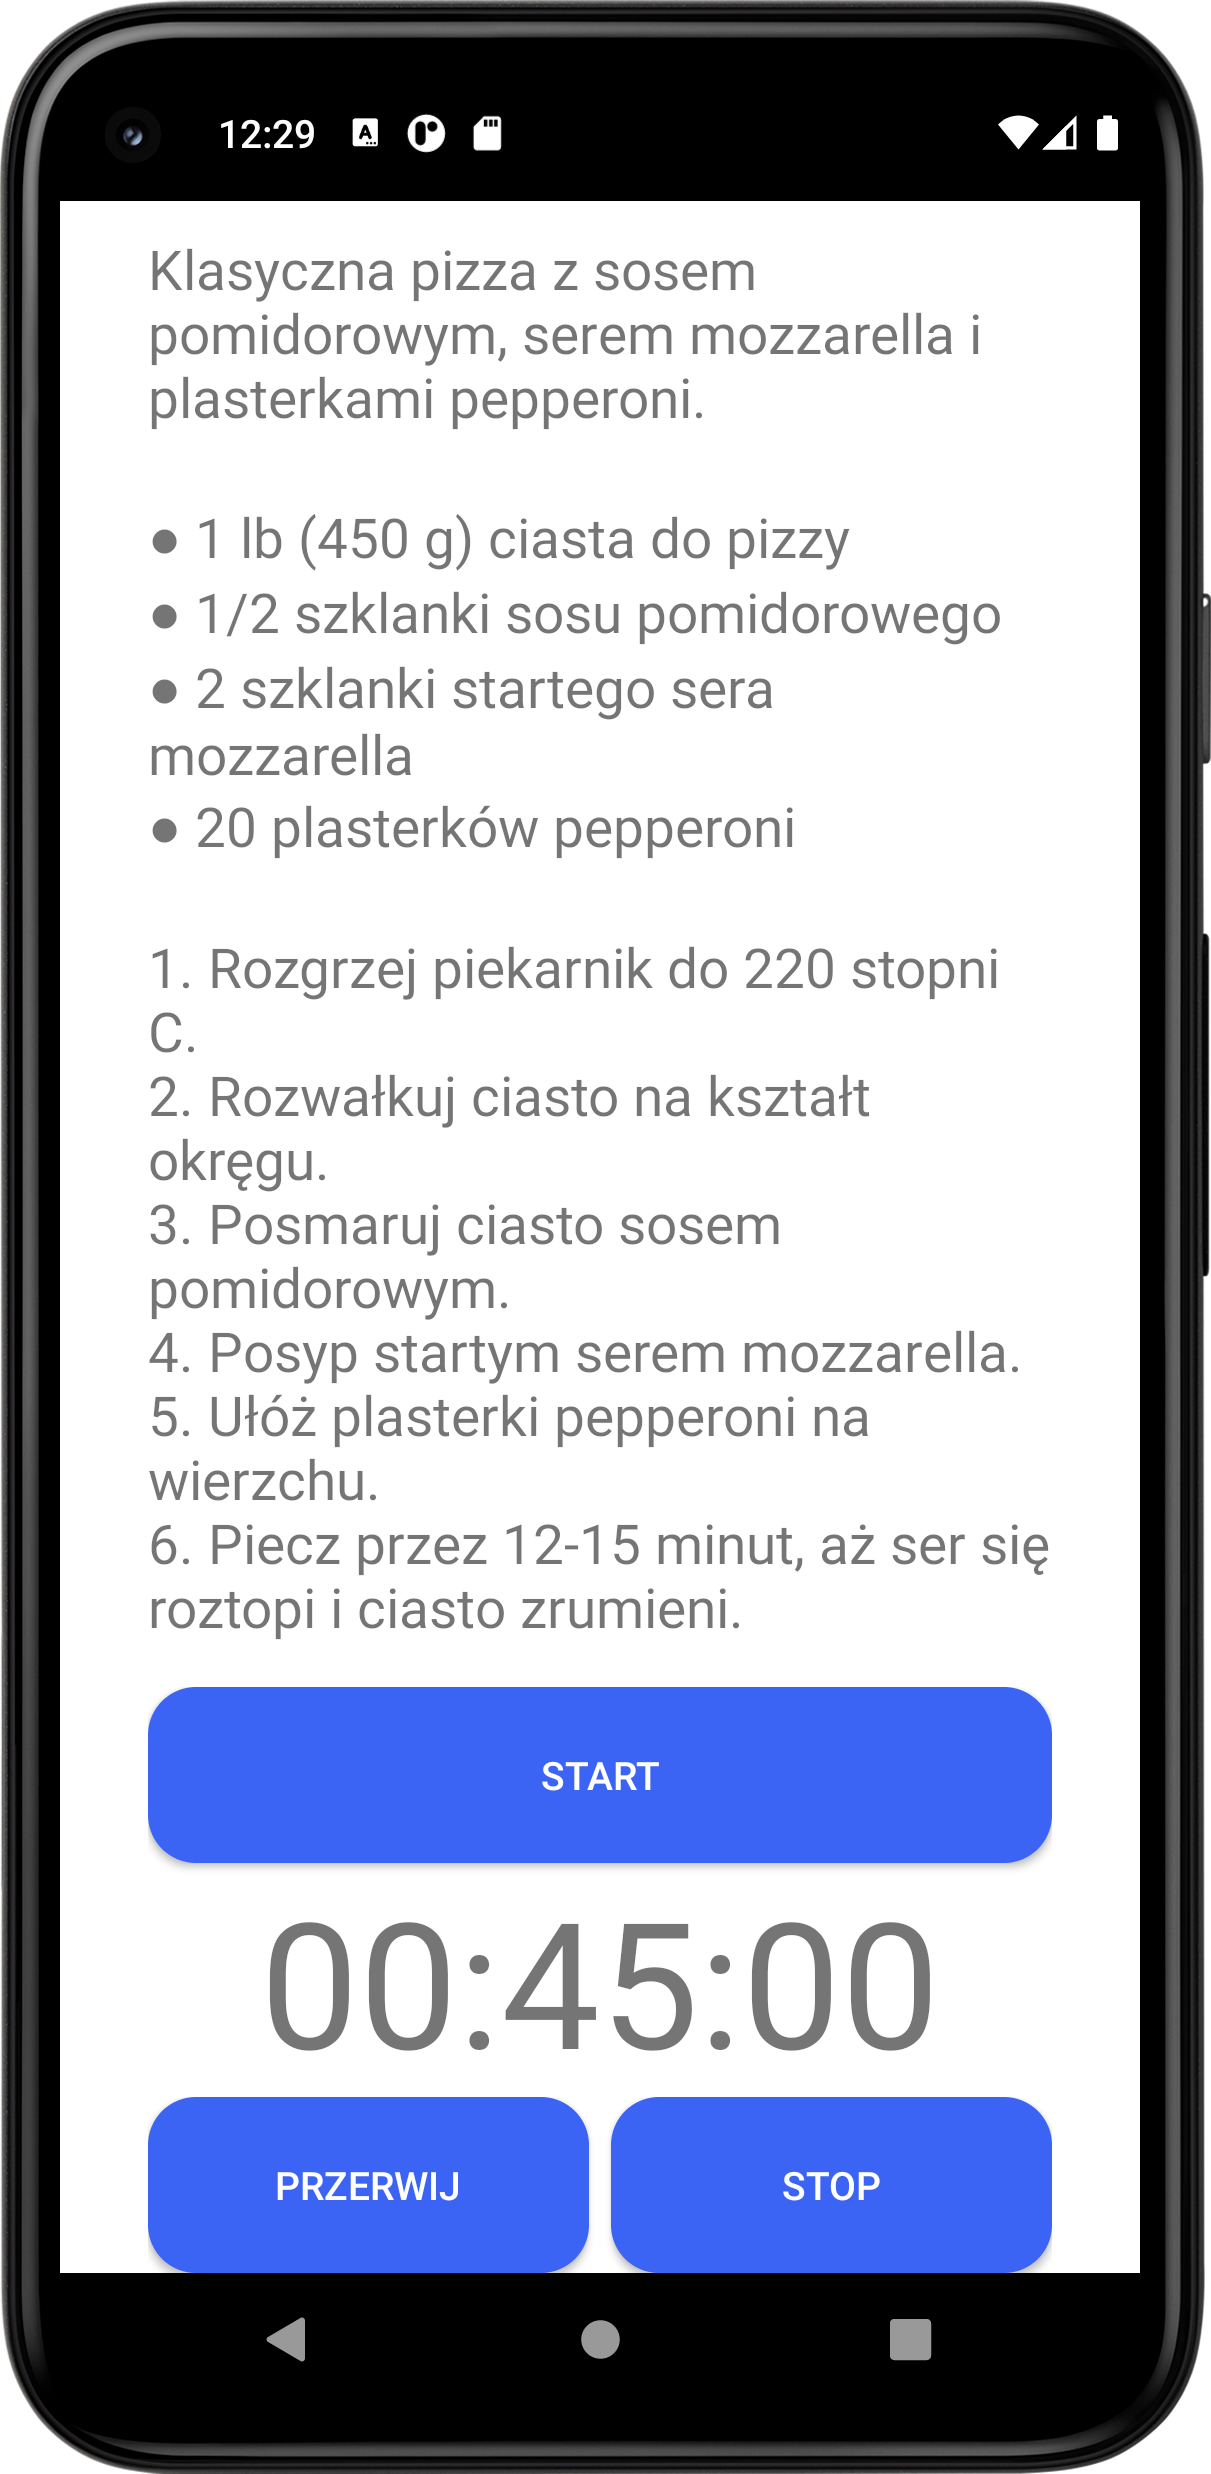
\includegraphics[width=0.4\textwidth]{../res/phone_timer}
    \captionof{figure}{Timer dla telefonu}
\end{figure}

\newpage

\begin{mylisting}
class TimerFragment : Fragment() {
    private var _binding: FragmentTimerBinding? = null
    private val binding get() = _binding!!
    private lateinit var startButton: AppCompatButton
    private lateinit var resetTimerButton: AppCompatButton
    private lateinit var stopButton: AppCompatButton
    private lateinit var timerValue: TextView
    private var isTimerRunning: Boolean = false
    private var time: Long = 0L
    private var timeRemaining: Long = 0L
    private var timer: CountDownTimer? = null

    override fun onCreate(savedInstanceState: Bundle?) {
        super.onCreate(savedInstanceState)

        val totalTime = arguments?.getString("total_time")

        if (totalTime != null) {
            time = totalTime.toLong() * 60000
        }
        timeRemaining = time
    }

    override fun onCreateView(
        inflater: LayoutInflater, container: ViewGroup?,
        savedInstanceState: Bundle?,
    ): View {
        _binding = FragmentTimerBinding.inflate(inflater, container, false)
        val rootView = binding.root

        startButton = binding.startTimerButton
        stopButton = binding.stopTimerButton
        resetTimerButton = binding.resetTimerButton
        timerValue = binding.timerValue

        val initialTime = time / 1000
        if (!isTimerRunning) {
            timerValue.text = String.format(
                "%02d:%02d:%02d",
                initialTime / 3600,
                (initialTime % 3600) / 60,
                initialTime % 60
            )
        }
\end{mylisting}
\newpage
\begin{enumerate}
    \item Przycisk start
\begin{mylisting}
startButton.setOnClickListener {
        if (!isTimerRunning) {
            timer = object : CountDownTimer(timeRemaining, 1000L) {
                override fun onTick(millisUntilFinished: Long) {
                    timeRemaining = millisUntilFinished
                    updateTimerText()
                }

                override fun onFinish() {
                    startVibrations()
                    isTimerRunning = false
                    updateTimerText()
                    timeRemaining = time
                }
            }

            timer?.start()
            isTimerRunning = true
        } else {
            timer = object : CountDownTimer(timeRemaining, 1000L) {
                override fun onTick(millisUntilFinished: Long) {
                    timeRemaining = millisUntilFinished
                    updateTimerText()
                }

                override fun onFinish() {
                    startVibrations()
                    isTimerRunning = false
                    updateTimerText()
                    timeRemaining = time
                }
            }
            timer?.start()
        }
    }
\end{mylisting}

\item Osiągnięcie wartości zerowej jest sygnalizowane wibracjami.

\newpage
\item Przycisk stop i  reset

\begin{mylisting}
stopButton.setOnClickListener {
    onStop()
}

resetTimerButton.setOnClickListener {
    resetTimer()
}


override fun onStop() {
    super.onStop()
    if (isTimerRunning) {
        timer?.cancel()
        timer = null
    }
}

private fun resetTimer() {
    if (isTimerRunning) {
        timer?.cancel()
        timeRemaining = 0L
        updateTimerText()
        timer = null
        timeRemaining = time
    }
}
\end{mylisting}
\end{enumerate}

\newpage

\item Elementy biblioteki wsparcia wzornictwa
\begin{enumerate}
    \item Fragment z kategoriami przepisów działa analogicznie do listy przepisów
     tylko jest on 
    przekazywany do GridLayoutManager.
\begin{mylisting}
private fun setupCategoryRecyclerView(
    recyclerView: RecyclerView,
    itemListFragmentContainer: View?,
) {
    RetrofitInstance.api.getCategories().enqueue(object : Callback<List<Category>> {
        override fun onResponse(
            call: Call<List<Category>>,
            response: Response<List<Category>>,
        ) {
            if (response.isSuccessful && response.body() != null) {
                val categories = (response.body())!!

                for (category in categories) {
                    Log.e(ContentValues.TAG, category.name)
                }

                val gridNum = 2;
                val layoutManager = GridLayoutManager(recyclerView.context, gridNum)

                recyclerView.layoutManager = layoutManager
                recyclerView.adapter = CategoryRecyclerViewAdapter(
                    categories, itemListFragmentContainer
                )
            } else {
                Log.e(ContentValues.TAG, response.code().toString())
                Log.e(ContentValues.TAG, "Response not successful")
            }
        }

        override fun onFailure(call: Call<List<Category>>, t: Throwable) {
            Log.e(ContentValues.TAG, "Response not successful")
            Log.e(ContentValues.TAG, t.message.toString())
        }
    })
}
\end{mylisting}

    \end{enumerate}

\newpage

\item Elementy biblioteki wsparcia wzornictwa


\begin{enumerate}
    \item Karty kategorii zamiast listy nazw potraw używają 
    widoku RecyclerView z układem siatki (grid), 
    w którym poszczególne pozycje (potrawy) są prezentowane 
    w postaci obrazka i nazwy, dla których użyto widoku CardView. 

    \begin{figure}[ht]
        \centering
        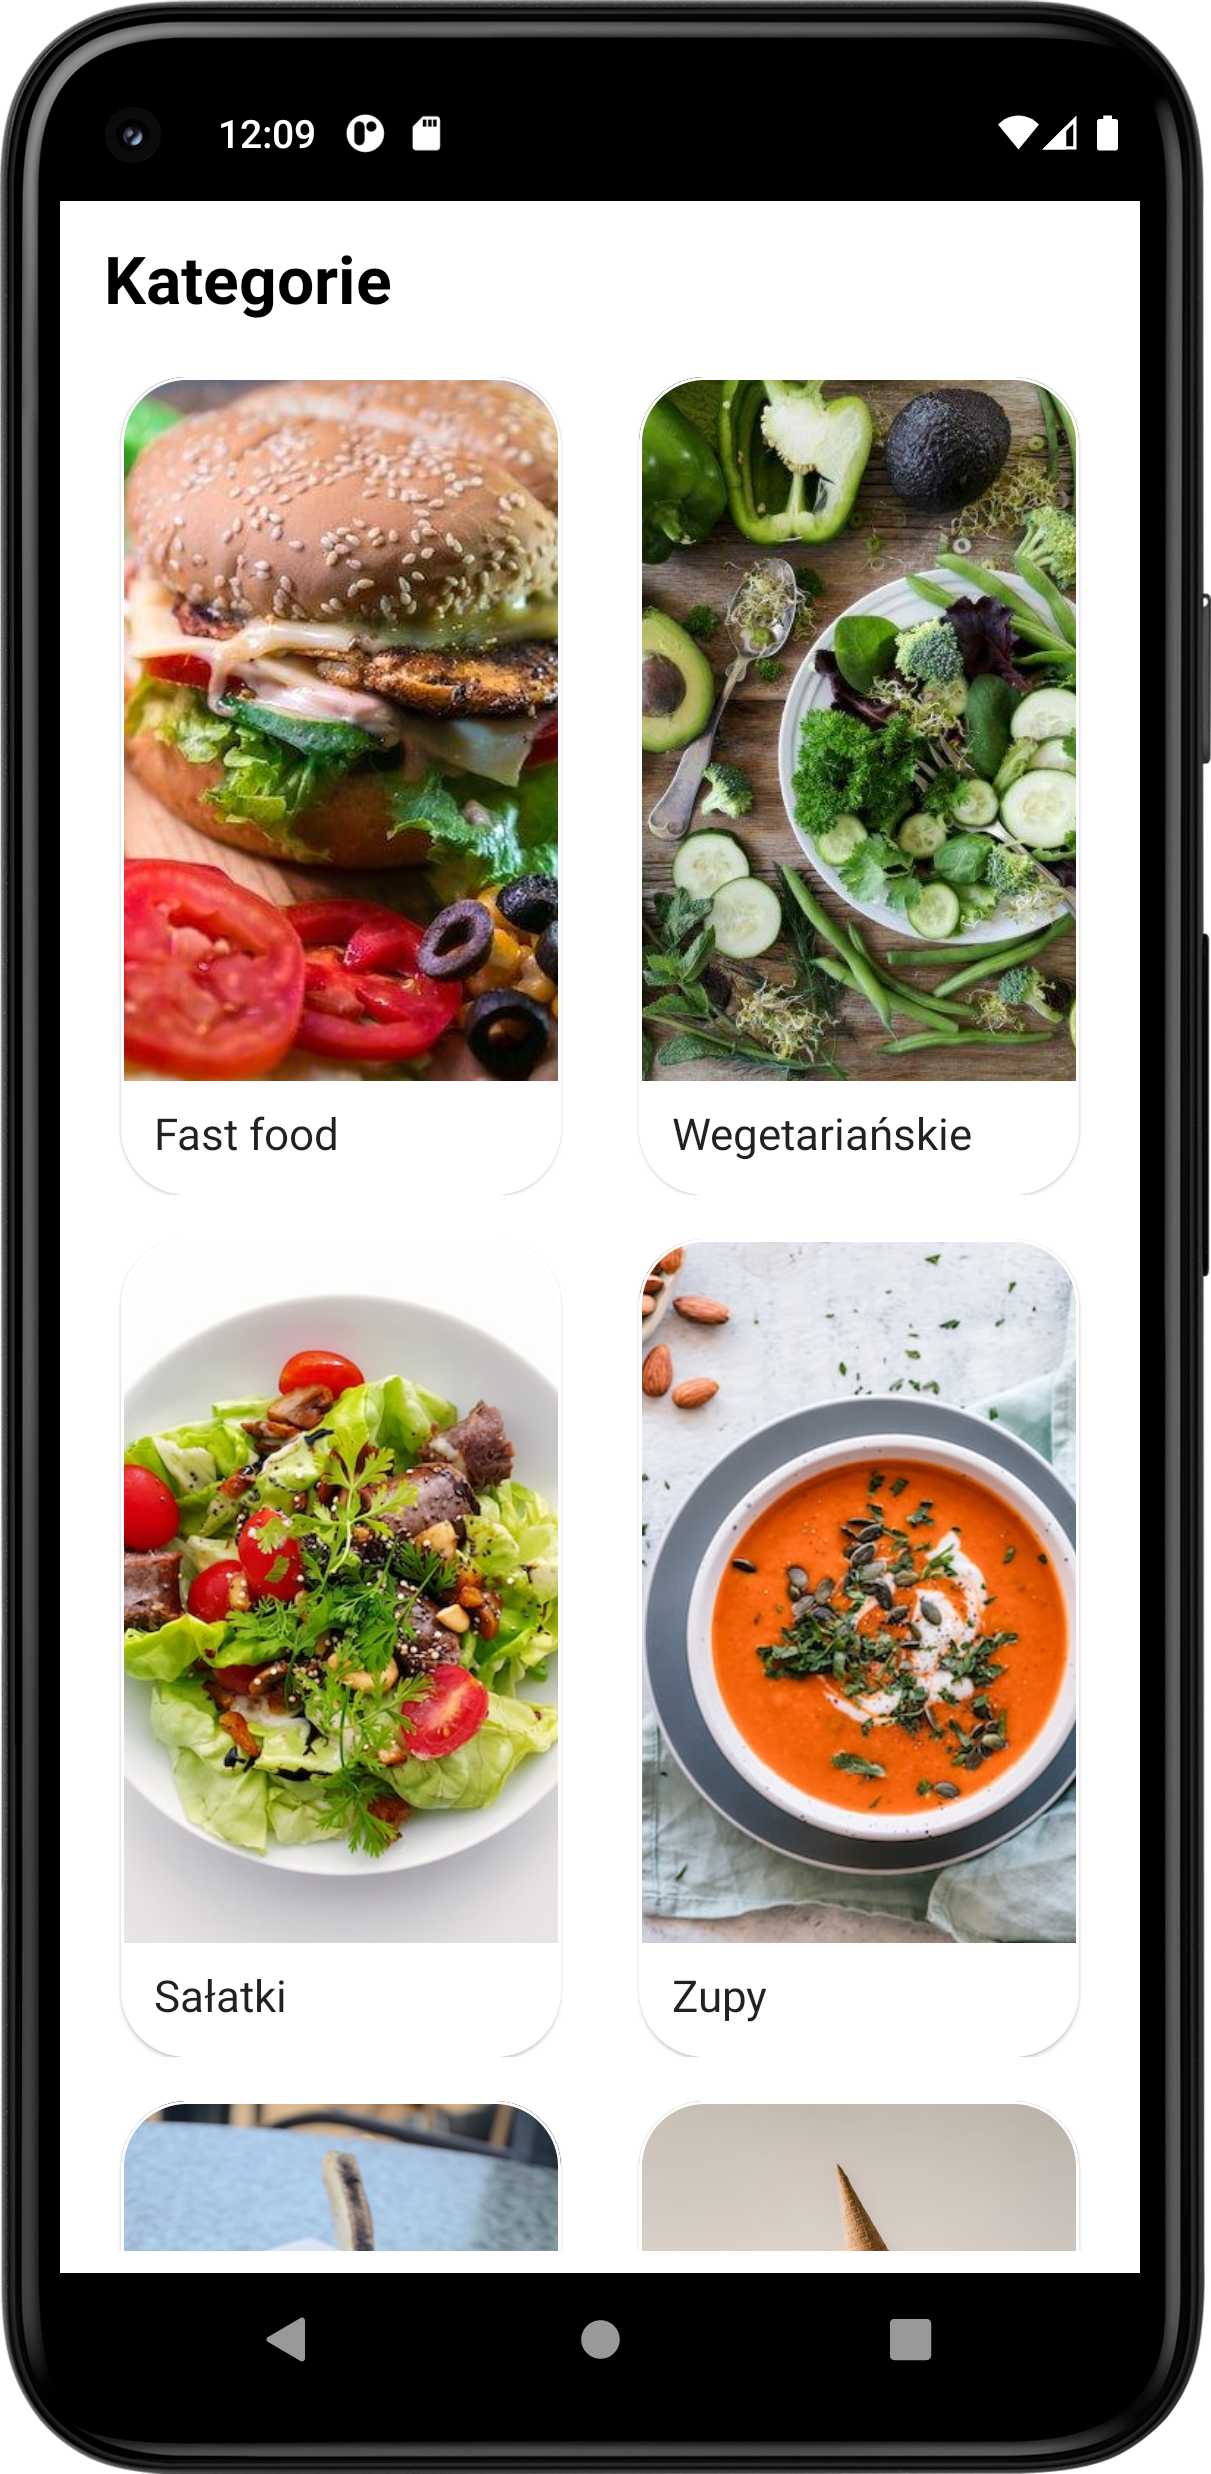
\includegraphics[width=0.4\textwidth]{../res/category_view}
        \captionof{figure}{Widok kategorii}
    \end{figure}
\newpage

Karta kategorii z widokiem MaterialCardView
\begin{mylisting}
<com.google.android.material.card.MaterialCardView
    android:layout_width="160dp"
    android:layout_height="wrap_content"
    app:cardCornerRadius="24dp"
    app:layout_constraintBottom_toBottomOf="parent"
    app:layout_constraintLeft_toLeftOf="parent"
    app:layout_constraintRight_toRightOf="parent"
    app:layout_constraintTop_toTopOf="parent"
    app:strokeColor="?attr/colorOnPrimaryContainer"
    app:strokeWidth="1dp">

    <RelativeLayout
        android:layout_width="match_parent"
        android:layout_height="wrap_content"
        android:gravity="center">

        <ImageView
            android:id="@+id/item_image"
            android:layout_width="160dp"
            android:layout_height="256dp"
            android:contentDescription="@string/category_image"
            android:scaleType="centerCrop" />

        <TextView
            android:id="@+id/item_number"
            android:layout_width="match_parent"
            android:layout_height="wrap_content"
            android:layout_below="@id/item_image"
            android:layout_marginStart="12dp"
            android:layout_marginTop="8dp"
            android:layout_marginEnd="8dp"
            android:layout_marginBottom="12dp"
            android:textAppearance="?attr/textAppearanceListItem" />

    </RelativeLayout>
</com.google.android.material.card.MaterialCardView>
\end{mylisting}

    \newpage
    \item Na ekranie szczegółów pojawia się przycisk FAB, który odświeża listę 
    i pokazuje komunikat "Updating recipes...".
    
    \begin{mylisting}
override fun onViewCreated(view: View, savedInstanceState: Bundle?) {
    super.onViewCreated(view, savedInstanceState)

    val recyclerView: RecyclerView = binding.itemList
    val itemDetailFragmentContainer: View? = view.findViewById(R.id.item_detail_nav_container)

    val backButton: ImageView = view.findViewById(R.id.back_button)
    backButton.setOnClickListener {
        requireActivity().onBackPressed()
    }
    val fab: FloatingActionButton = view.findViewById(R.id.fab)

    fab.setOnClickListener {
        val message = "Updating recipes..."
        val context = requireContext()
        context.toast(message)
        fetchRecipesByCategory(category, recyclerView, itemDetailFragmentContainer)
    }

    setupRecyclerView(recyclerView, itemDetailFragmentContainer)
}
    \end{mylisting}

    \newpage
    \item Ekran z opisem aplikacji i zmiana mechanizmów nawigacji.
    Przechodzenie pomiędzy kartami odbywa się za pomocą gestu przeciągnięcia.
    
    \begin{figure}[ht]
        \centering
        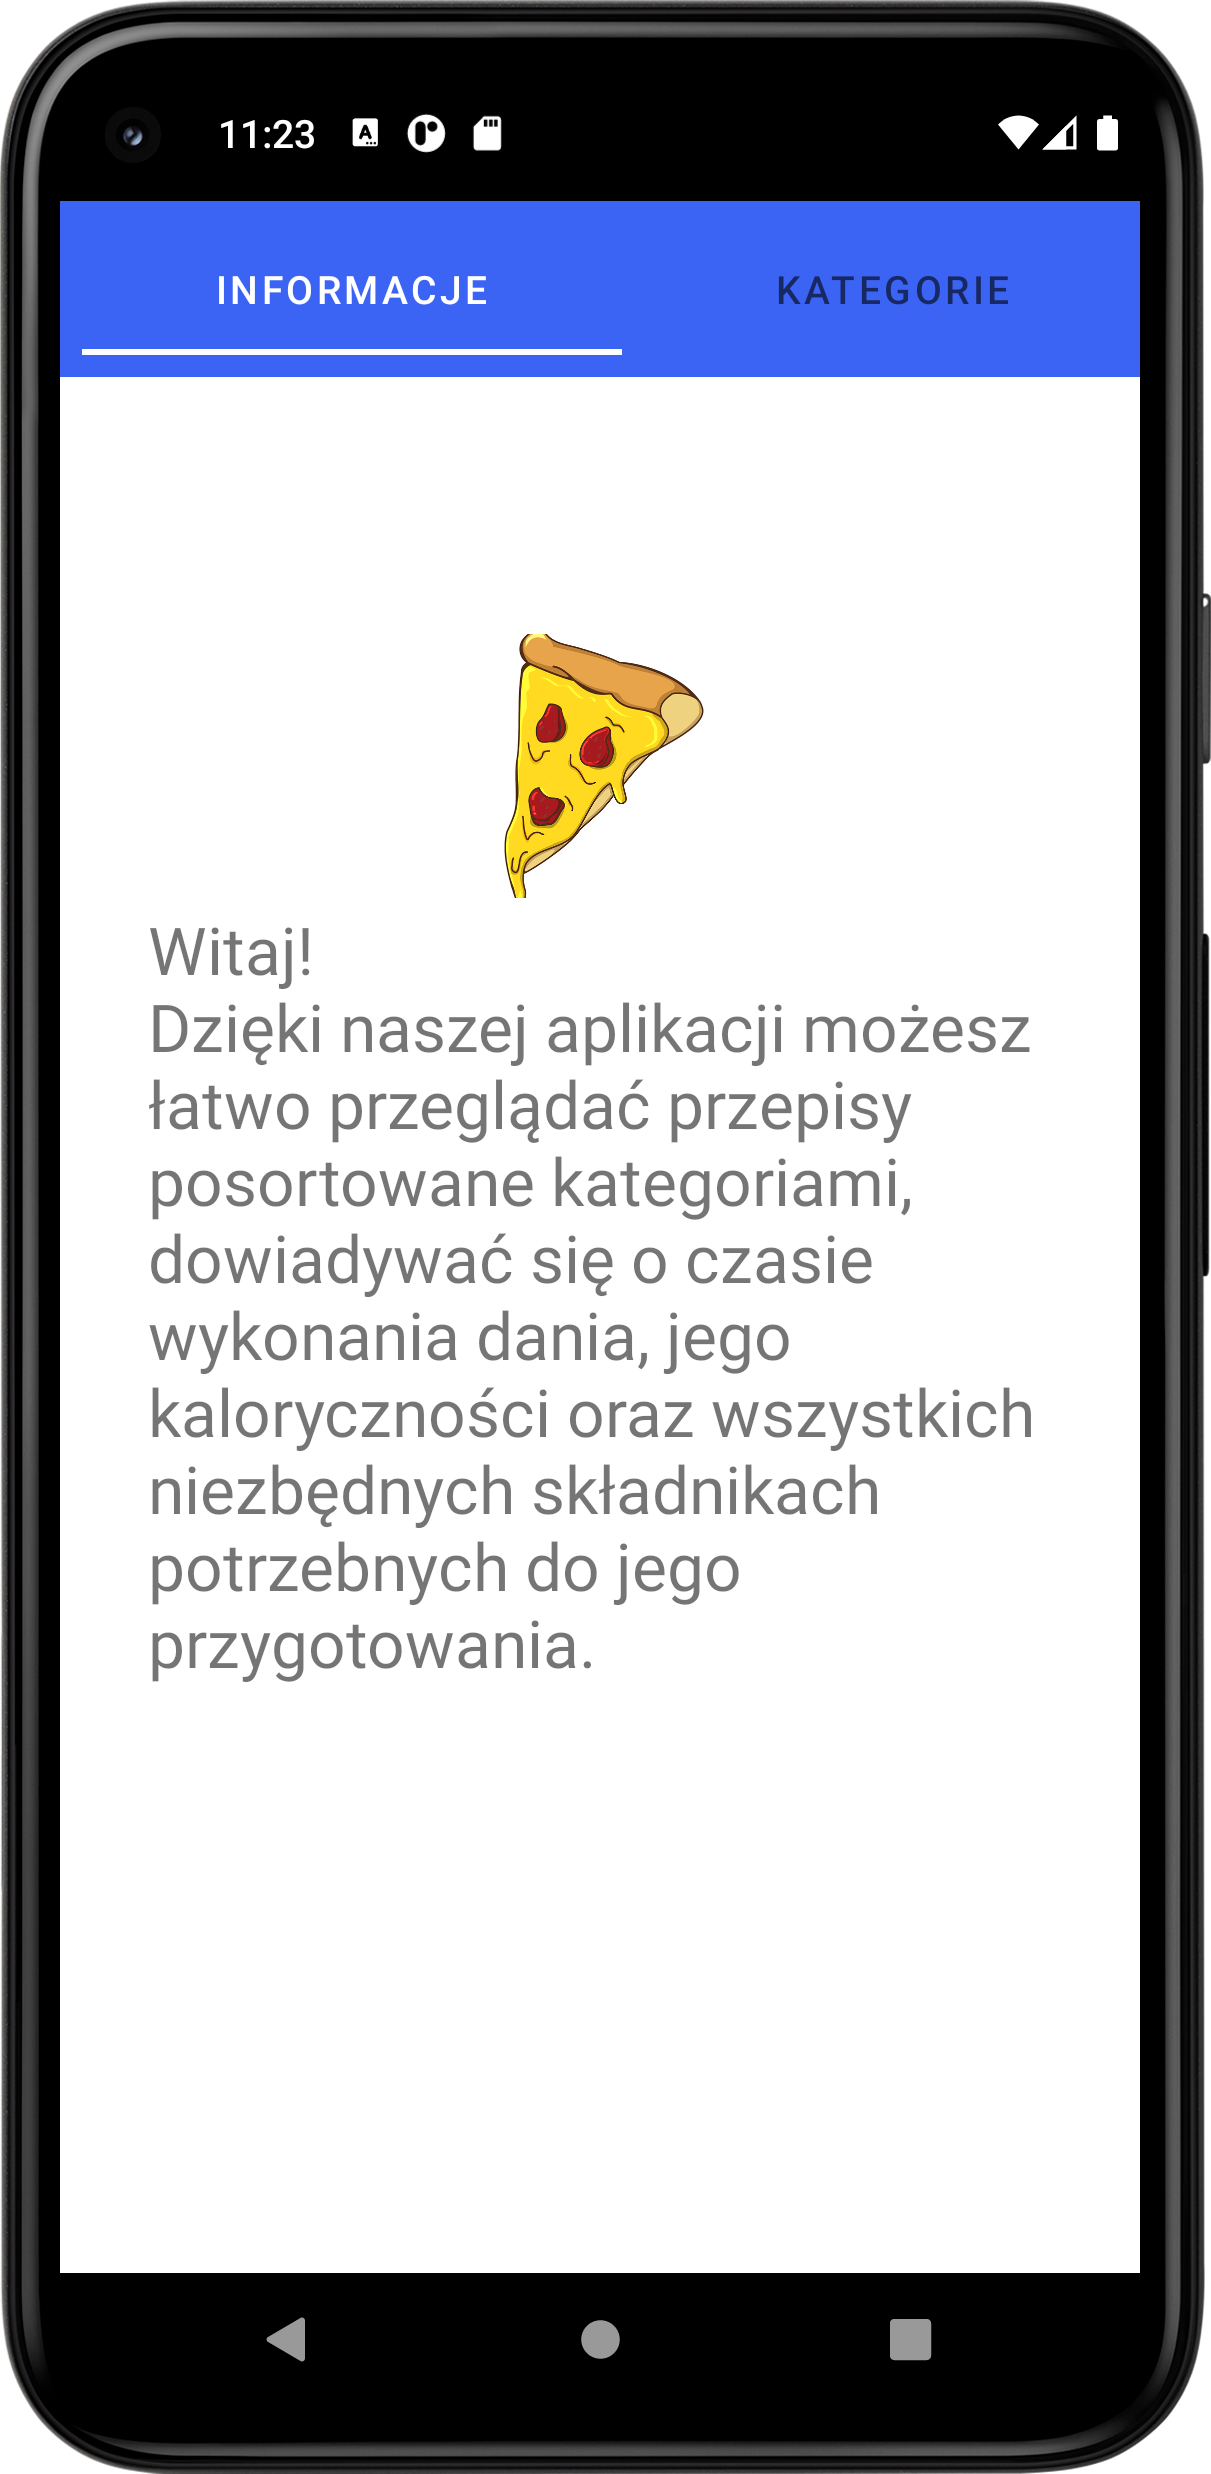
\includegraphics[width=0.4\textwidth]{../res/app_info}
        \captionof{figure}{Opis aplikacji}
    \end{figure}

\end{enumerate}

\item Animacje
\begin{enumerate}
    \item Podczas uruchomienia aplikacji pojawia się prosta animacja 
    obrazka nad opisem aplikacji.
\end{enumerate}

\end{enumerate}


\end{document}
